\documentclass[a4paper, 11pt, notitlepage, english]{article}

\usepackage{babel}
\usepackage[utf8]{inputenc}
\usepackage[T1]{fontenc, url}
\usepackage{textcomp}
\usepackage{amsmath, amssymb}
\usepackage{amsbsy, amsfonts}
\usepackage{graphicx, color}
\usepackage{parskip}
\usepackage{framed}
\usepackage{amsmath}
\usepackage{xcolor}
\usepackage{multicol}
\usepackage{url}
\usepackage{flafter}
\usepackage{caption}

%\DeclareCaptionLabelSeparator{colon}{. }
\renewcommand{\captionfont}{\sffamily}
\renewcommand{\captionlabelfont}{\bf\sffamily}
\setlength{\captionmargin}{40pt}

\usepackage{geometry}
\geometry{headheight=0.01mm}
\geometry{top=24mm, bottom=29mm, left=39mm, right=39mm}

\renewcommand{\arraystretch}{2}
\setlength{\tabcolsep}{10pt}
\makeatletter
\renewcommand*\env@matrix[1][*\c@MaxMatrixCols c]{%
  \hskip -\arraycolsep
  \let\@ifnextchar\new@ifnextchar
  \array{#1}}
%
% Parametere for inkludering av kode fra fil
%
\usepackage{listings}
\lstset{language=python}
\lstset{basicstyle=\ttfamily\small}
\lstset{frame=single}
\lstset{keywordstyle=\color{red}\bfseries}
\lstset{commentstyle=\itshape\color{blue}}
\lstset{showspaces=false}
\lstset{showstringspaces=false}
\lstset{showtabs=false}
\lstset{breaklines}

%
% Definering av egne kommandoer og miljøer
%
\newcommand{\dd}[1]{\ \text{d}#1}
\newcommand{\f}[2]{\frac{#1}{#2}} 
\newcommand{\beq}{\begin{equation}}
\newcommand{\eeq}{\end{equation}}
\newcommand{\bra}[1]{\langle #1|}
\newcommand{\ket}[1]{|#1 \rangle}
\newcommand{\braket}[2]{\langle #1 | #2 \rangle}
\newcommand{\braup}[1]{\langle #1 \left|\uparrow\rangle\right.}
\newcommand{\bradown}[1]{\langle #1 \left|\downarrow\rangle\right.}
\newcommand{\av}[1]{\left| #1 \right|}
\newcommand{\op}[1]{\hat{#1}}
\newcommand{\braopket}[3]{\langle #1 | {#2} | #3 \rangle}
\newcommand{\ketbra}[2]{\ket{#1}\bra{#2}}
\newcommand{\pp}[1]{\frac{\partial}{\partial #1}}
\newcommand{\ppn}[1]{\frac{\partial^2}{\partial #1^2}}
\newcommand{\up}{\left|\uparrow\rangle\right.}
\newcommand{\upup}{\left|\uparrow\uparrow\rangle\right.}
\newcommand{\down}{\left|\downarrow\rangle\right.}
\newcommand{\downdown}{\left|\downarrow\downarrow\rangle\right.}
\newcommand{\updown}{\left|\uparrow\downarrow\rangle\right.}
\newcommand{\downup}{\left|\downarrow\uparrow\rangle\right.}
\newcommand{\bupup}{\left.\langle\uparrow\uparrow\right|}
\newcommand{\bdowndown}{\left.\langle\downarrow\downarrow\right|}
\newcommand{\bupdown}{\left.\langle\uparrow\downarrow\right|}
\newcommand{\bdownup}{\left.\langle\downarrow\uparrow\right|}
\renewcommand{\d}{{\rm d}}
\newcommand{\Res}[2]{{\rm Res}(#1;#2)}
\newcommand{\To}{\quad\Rightarrow\quad}
\newcommand{\eps}{\epsilon}
\newcommand{\inner}[2]{\langle #1 , #2 \rangle}


\newcommand{\bt}[1]{\boldsymbol{#1}}
\newcommand{\mat}[1]{\textsf{\textbf{#1}}}
\newcommand{\I}{\boldsymbol{\mathcal{I}}}
\newcommand{\p}{\partial}
%
% Navn og tittel
%
\author{Jonas van den Brink \\ \texttt{j.v.d.brink@fys.uio.no}}
\title{MAT-INF3360 \\ Mandatory Exercises 1}

\begin{document}
\maketitle
\section*{Exercise 2.30}
In this exercise we will show the orthogonality relation between the discrete eigenfunctions of the operator $L_h$, which is defined as the negative of a 2.\ order central difference, meaning we have:
$$L_h v(x_j) = \frac{-v(x_{j+1}) + 2v(x_j) - v(x_{j-1})}{h^2}.$$
So we are studying the functions $v \in D_{h,0}$ that satisfy the eigenvalue problem
$$L_h v = \mu v.$$
From the text we know that the eigenstates are:
$$v_k(x_j) = \sin(k\pi x_j) \mbox{ for } k=1,2,\ldots,n.$$
And we will show the orthogonality
$$\langle v_n, v_m\rangle_h = \delta_{n,m}/2,$$
where $\delta_{n,m}$ denotes the Kronecker-delta.

\subsection*{a)}
We will show that the sum
$$S_k = \sum_{j=0}^n \cos(k\pi x_j),$$
is $S_k = 0$ for $k$ even, and $S_k=1$ if $k$ is odd. For $k=0$ the sum is trivial and obviously equal to $n+1$.

We start by writing the cosine term into a linear combination of expoentials with a purely imaginary argument and splitting the sum into parts
$$\sum_{j=0}^n \cos(k\pi x_j) = \frac{1}{2}\bigg(\sum_{j=0}^n \exp(ik\pi x_j)+ \sum_{j=0}^n \exp(-ik\pi x_j)\bigg).$$
by introducing the step size $h$ through $x_j = h\cdot j$, we can rewrite these sums as finite geometric sums, to which the value is known\footnote{See for example \emph{Rottman} page 112.}. We have
$$\sum_{j=0}^n \exp(\pm ik\pi x_j) = \sum_{j=0}^n [\exp(\pm ik\pi h)]^j = \frac{1-[\exp(\pm ik\pi h)]^{n+1}}{1 - \exp(\pm ik\pi h)}.$$
So our sum can be written
$$S_k = \frac{1}{2}\bigg(\frac{1-[\exp(ik\pi h)]^{n+1}}{1 - \exp(ik\pi h)} + \frac{1-[\exp(- ik\pi h)]^{n+1}}{1 - \exp(- ik\pi h)}\bigg).$$
Now we use the fact that
$$[\exp(\pm ik\pi h)]^{n+1} = \exp(\pm ik\pi h (n+1)) = \exp(\pm ik\pi) = (-1)^k.$$
Due to the fact that $h(n+1)=1$. 

We now expand the latter fraction by $\exp(ik\pi h)$ and add the two fractions together to get
$$S_k = \frac{1}{2}\frac{1-\exp(ik\pi h) - (-1)^k(1 - \exp(ik\pi h))}{1 - \exp(ik\pi h)} = \frac{1 - (-1)^k}{2}.$$
And from this expression we readily see that
$$S_k = \begin{cases}
    0 & \mbox{for $k$ even} \\
    1 & \mbox{for $k$ odd}.\\
\end{cases}$$

\subsection*{b)}
We now turn to the inner-product, and will first show the orthogonality property of the discrete eigenfunctions $v_k$. Remebering that the inner product in the space $D_{h,0}$ is defined
$$\langle u,v\rangle_h = h\sum_{j=1}^n u_j v_j,$$
we can write the inner product as
$$\langle v_k, v_m \rangle_h = h\sum_{j=0}^n \sin(k\pi x_j)\sin(m\pi x_j).$$
Note that we let $j$ run from 0 and not 1, this is ok as $v_k(x_0) = 0$ for all $k$ anyway, so it doesn't affect the sum. 

Now, using the trigonometric identity
$$\sin(x)\sin(y) = \frac{1}{2}\big(\cos(x-y) - \cos(x+y)\big),$$
we can rewrite this sum as
$$\langle v_k, v_m \rangle_h = \frac{h}{2}\bigg(\sum_{j=0}^n \cos((k-m)\pi x_j) - \sum_{j=0}^n \cos((k+m)\pi x_j)\bigg),$$
which using the results of exercise a) can be written as
$$\langle v_k, v_m \rangle_h = \frac{h}{2}\bigg(S_{(k-m)} - S_{(k+m)}\bigg).$$
We now see that for any integer values of $k$ and $m$, both the difference $k-m$ and the sum $k+m$ will either be odd or even, and so the two sums cancel out, and we have
$$\langle v_k, v_m \rangle_h = 0 \mbox{ when }k\neq m.$$
When $k=m$, the first sum becomes $S_0 = n+1$, and so this result does \emph{not} apply to that case.

\subsection*{c)}
We now look at the case
$$\langle v_k, v_k \rangle_h.$$
Using the same steps as in the previous exercise we can show that this is equal to
$$\langle v_k, v_k \rangle_h = \frac{h}{2}\bigg(S_0 - S_{2k}\bigg).$$
From exercise a), we know that $S_{2k} = 0$ as $2k$ is even for all non-zero integers $k$, and we also know that $S_0 = n+1 = 1/h.$ Using this we have
$$\langle v_k, v_k \rangle_h = \frac{1}{2}.$$

And we have thus shown that
$$\langle v_k, v_m \rangle_h = \delta_{k,m}/2 \mbox{ q.e.d.}$$

\clearpage


\section*{Project 2.1}

We will be studying the problem
$$-u''(x) = f(x), \qquad x \in (0,1), \qquad u(0)=u(1)=0.$$
Which has solutions on the form
$$u(x) = x\int_0^1 (1-y)f(y)\, \d y - \int_0^x (x-y)f(y)\, \d y.$$
We will be looking at numerical schemes that result from using numerical approximations to the integrations in this form.

\subsection*{(a) The Trapezoidal Rule}
The trapezoidal rule is an intutive approximation to a definite integral. It is most easily understood from a geometric perspective. The definite integral 
$$I = \int_a^b F(x) \, \d x,$$
is the area under the curve $F(x)$ between the limits $a$ and $b$. The trapezoidal rule approximates this area as many small trapezoids, from which the area is easily calculated. See figure \ref{fig:trap} and \ref{fig:trap_se} for illustrations. 

Using more trapezoids should give a better approximation, but will also require more samplings. Using $n+1$ trapezoids, means using $n+2$ mesh points and thus $n+2$ samplings of the function $F(x)$.

Looking at figure \ref{fig:trap_se}, it is easy to see that the area of a single trapezoid is
$$a_i = (x_{i+1}-x_{i})\frac{F(x_{i+1}) + F(x_i)}{2}.$$
Here, the width of the trapezoid is given as $x_{i+1}-x_{i}$, which is the general case. In this project however, we will assume uniformely spaced mesh points, meaning we use
$$x_{i} = a + ih, \qquad h = x_{i+1}-x_i = \frac{b-a}{n+1}.$$
Summing over all the trapezoids, we see that all the internal mesh points are added twice, while the endpoints are added just once, we thus have
$$I = \int_a^b F(x) \, \d x \approx h\bigg( \frac{F(a)+F(b)}{2} + \sum_{i=1}^n F(x_i)\bigg).$$

\begin{figure}[p]
    \centering
    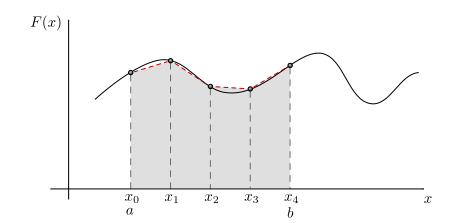
\includegraphics[width=\textwidth]{trapezoid}
    \caption{Illustration of using the trapezoidal rule to approximate an integral using 4 trapezoids, meaning we have $n=3$ internal mesh points \label{fig:trap}}
\end{figure}
\begin{figure}[p]
    \centering
    \includegraphics[width=\textwidth]{singleelement}
    \caption{A single trapezoid element. \label{fig:trap_se}}
\end{figure}

\clearpage

\subsection*{(b) Writing a Trapezoidal Integration Function}
We will now implement a procedure that for a given $a$, $b$, $F(x)$ and $n$ computes the approximation given by the trapezoidal rule. 

For simplicity, we write the code in Python:

\begin{lstlisting}
def trapez(F,a,b,n):
    h = (b-a)/(n+1)

    s = F(a)/2. + F(b)/2.
    for i in range(n):
        x += h
        s += F(x)
    
    return s*h
\end{lstlisting}
Note that this function is not very efficient. For practical use, it should either be vectorized using numpy or implemented in some other language, like for example C++.


\subsection*{(c)}
We now set $F(x) = x^5$ and $G(x) = \sqrt{|x-\frac{1}{2}|}$ and will compute the integrals
$$I_1 = \int_0^1 F(x) \, \d x \qquad \mbox{and} \qquad I_2 = \int_0^1 G(x)\, \d x,$$
using the trapezoidal rule. We first compute them analytically, so that we have an exact solution to compare our results to.

The first integral is trivial
$$I_1 = \int_0^1 x^5 \, \d x = \frac{1}{6}.$$
The second integral can be solved by realizing it is symetric about $x=1/2$, and substituting $u=x-1/2$:
$$I_2 = \int_0^1 \sqrt{|x-\frac{1}{2}}\,\d x = 2\int_0^{\frac{1}{2}} \sqrt{u}\, \d u = \frac{\sqrt{2}}{3}.$$


Using the function \verb+trapez(F,a,b,n)+ defined above, we calculate numerical approximations to $I_1$ and $I_2$ using $n=10,20,40,80,160$ internal mesh points.

To estimate the rate of convergence for the approximations of these integrals, we assume that the error is proportional to some order of the step length $h$:
$$e_h = ch^r,$$
where $c$ is a proportionality constant. To find $r$, we compare for two different values of $h$
$$r = \frac{\ln(e_{h_1}/e_{h_2})}{\ln(h_1/h_2)}.$$

The results are shown in table \ref{table:trapez}.

\begin{table}
\centering
    \begin{tabular}{c|c|c|c|c}
        $n$ & Rel.\ error $I_1$ & Conv.\ rate $I_2$ & Rel.\ error $I_2$ & Conv.\ rate $I_2$\\ \hline
10  & 2.06$\cdot 10^{-2}$ &  & 9.15$\cdot 10^{-3}$ \\ \hline
20  & 5.67$\cdot 10^{-3}$ & 1.9981  & 3.25$\cdot 10^{-3}$  & 1.5995\\ \hline
40  & 1.49$\cdot 10^{-3}$ & 1.9995  & 1.13$\cdot 10^{-3}$  & 1.5760\\ \hline
80  & 3.81$\cdot 10^{-4}$ & 1.9999  & 3.92$\cdot 10^{-4}$  & 1.5567\\ \hline
160 & 9.64$\cdot 10^{-5}$ & 2.0000 & 1.36$\cdot 10^{-4}$   & 1.5417 \\ 
    \end{tabular}
    \caption{Results of using the \texttt{trapez} function to evalute the integrals of $F(x)$ and $G(x)$ on the unit interval.\label{table:trapez}}
\end{table}

\clearpage

\subsection*{(d)}
We now define the functions
$$\alpha(x) = \int_0^x f(y) \, \d y \qquad \mbox{and} \qquad \beta(x) = \int_0^x yf(y) \, \d y.$$
And will use these to redwrite the general solution to our boundary value problem
$$u(x) = x\int_0^1 (1-y)f(y)\, \d y - \int_0^x (x-y)f(y)\, \d y.$$
Divding the integrals makes this an easy task
$$u(x) = x\bigg(\underbrace{\int_0^1 f(y) \, \d y}_{\alpha(1)} - \underbrace{\int_0^1 y f(y) \, \d y}_{\beta(1)}\bigg) + \underbrace{\int_0^x yf(y)\, \d y}_{\beta(x)} - x \underbrace{\int_0^x f(y)\, \d y}_{\alpha(x)}.$$
So we see that we can write the solution as
$$u(x) = x\big(\alpha(1)-\beta(1)\big) + \beta(x) - x\alpha(x) \quad \mbox{q.e.d.}$$

\clearpage

\subsection*{(e)}
We will now find approximations to $\alpha(x_i)$ and $\beta(x_i)$. Remember that 
$$\alpha(x_i) = \int_0^{x_i} f(y) \, \d y, \quad \beta(x_i) = \int_0^{x_i} y f(y) \, \d y \quad \mbox {where } x_i = ih.$$
We will also be using the shorthand $f(x_i) = f_i$. We start by realizing that if the value of $\alpha(x_i)$ is known, calculating the value of $\alpha(x_{i+1})$ can be simplified in the following manner:
$$\alpha(x_{i+1}) = \int_0^{x_{i+1}} f(y) \, \d y = \int_0^{x_i}f(y) \, \d y + \int_{x_i}^{x_{i+1}}f(y)\, \d y = \alpha(x_i) + \int_{x_i}^{x_{i+1}}f(y)\, \d y.$$
The integral from $x_i$ to $x_{i+1}$ can then be approximated with the trapezoidal rule, using one internal mesh point---as this mesh point will lie between $x_i$ and $x_{i+1}$ it is a kind of \emph{virtual} mesh point. We then have
$$\int_{x_i}^{x_{i+1}}f(y)\, \d y \approx \frac{h}{4}\big(f_i + 2f_{i+1/2} + f_{i+1}\big).$$
For simplicity, we let $\alpha_i$ denote the approximation to $\alpha(x_i)$ and \emph{not} the exact. We then have
$$\alpha_0 = 0, \qquad \alpha_{i+1} = \alpha_i + \frac{h}{4}\big(f_i + 2f_{i+1/2} + f_{i+1}\big).$$
For $\beta(x_i)$, we do the exact same steps, and find
$$\beta_0 = 0, \qquad \beta_{i+1} = \beta_i + \frac{h}{4}\big(x_if_i + 2x_{i+1/2}f_{i+1/2} + x_{i+1}f_{i+1}\big).$$

\subsection*{(f)}
As $\alpha(x_{n+1}) = \alpha(1) \approx \alpha_{n+1},$ we can define an approximation to the solution of the boundary value problem $u$ as:
$$u_i = x_i(\alpha_{n+1} - \beta_{n+1}) + \beta_i - x_i\alpha_i.$$
Note that as previously, $u_i$ is the discrete approximation in the point $x_i$, and not the exact solution evaluated in $x_i$. From our Dirichlet boundary conditions we also know that
$u_0 = u_{n+1} = 0.$

We will now implement this approximation on a computer. There is however one problem, in some cases, we might not be able to evaluate the source-term $f$ in the virtual point $x_{i+1/2}$, which is not a mesh point. In some cases, we will therefore have to approximate this value, using a mean
$$f_{i+1/2} \approx (f_i + f_{i+1})/2.$$
This is effectively the same as using the trapezoidal rule with no internal mesh points for the integral 
$$\int_{x_i}^{x_{i+1}} f(y)\, \d y.$$


\subsection*{g)}
$$\beta_{i+1} = \beta_i + \frac{h}{2}\big(x_if_i + 2x_{i+1/2}f_{i+1/2} + x_{i+1}f_{i+1}\big)$$

$$\beta_i - x_i\alpha$$


\begin{lstlisting}
from pylab import *


a[n+1] = a[i] + h/2*(f[i] + 2*f[i+0.5] + f[i+1])
b[n+1] = b[i] + h/2()

def boundary_value_problem_solver(f, n):
    u = zeros(n+2)
    a = zeros(n+2)
    b = zeros(n+2)
    x = linspace(0,1,n+2)
    h = x[1]-x[0]

    if callable(f):
        for i in range(n+1):
            a[i+1] = a[i] + h/2*(f(x[i] + 2*f(x[i]+h/2.) + f(x[i+1])
  
\end{lstlisting}

We now want to test our solver, and will do so for the following source terms
\begin{align*}
f(x) &= 1, \\
f(x) &= x,\\
f(x) &= x^2, \\
f(x) &= e^x, \\
f(x) &= \cos(ax) \mbox{ for }a\in\mathbb{R}.
\end{align*}
All of these are solvable, with known exact solutions, giving us a perfect chance to compare our numerical solution.

\end{document}
